\documentclass[tikz]{standalone}
\usepackage{physics}
\usetikzlibrary{decorations.pathmorphing,patterns}

\begin{document}
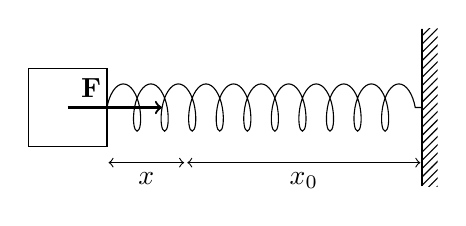
\begin{tikzpicture}
  %Wall
  \fill [pattern = north east lines] (5,-1) rectangle (5.2,1);
  \draw[thick] (5,1) -- (5,-1);

  %Spring
  \draw[decoration={aspect=0.4, segment length=3.5mm, amplitude=3mm,coil},decorate] (1,0) -- (5,0);

  %Box
  \draw (0,-0.5) rectangle (1,0.5);

  % Horizontal arrows displacements
  \draw[<->] (2+0.02,-0.7) -- (5-0.02,-0.7);
  \node[anchor=north] at (3.5, -0.7) {$x_0$};

  \draw[<->] (1+0.02,-0.7) -- (2-0.02,-0.7);
  \node[anchor=north] at (1.5, -0.7) {$x$};

  %Force
  \draw[->,thick] (0.5, 0) -- (1.7, 0);
  \node[anchor=south] at (0.8, 0) {$\vb{F}$};
\end{tikzpicture}
\end{document}